%\documentclass[a4paper,12pt,oneside,openright,final]{memoir} %twocolumn,
\documentclass[a4paper,12pt,oneside,openright]{memoir}

\let\footruleskip\undefined
\usepackage[utf8]{inputenc}
\usepackage[english]{babel}
\usepackage{etex}
\usepackage{times}
\DisemulatePackage{setspace}
\usepackage{setspace}
\usepackage{amssymb}
\usepackage{amsfonts}

\usepackage{graphicx}
\usepackage[printwatermark]{xwatermark}
% uncomment for watermarks
%\newwatermark[allpages,color=red!10,angle=45,scale=5,xpos=-15,ypos=30]{DRAFT}

\usepackage{alltt}
\usepackage{moreverb}
%for more info on hyperref package see http://en.wikibooks.org/wiki/LaTeX/Packages/Hyperref
\usepackage[pdftex,colorlinks=true,linkcolor=blue, citecolor=magenta]{hyperref}
\usepackage{eso-pic}
\usepackage{transparent}
\setlength{\columnsep}{3em}

\usepackage{tcolorbox}
\usepackage{listings}
\definecolor{codebgcolor}{HTML}{6E84D6}
\definecolor{codefgcolor}{HTML}{000000}% 071D70
\definecolor{basiccolor}{HTML}{000000}%1435AD
\definecolor{stringcolor}{HTML}{050505}% 2C3E82
\definecolor{highlight}{HTML}{FFB100}
\definecolor{annotationbgcolor}{HTML}{FFD473}

\usepackage{wrapfig}
\usepackage{caption}
\usepackage{subcaption}
\usepackage{alltt}
\usepackage{moreverb}
% tikz related packages to provide scalable graphics
\usepackage{tikz}
\usetikzlibrary{calc,mindmap,backgrounds,positioning,arrows,shapes,shapes.arrows,shapes.misc,automata,petri,patterns,scopes,chains,matrix,decorations.pathmorphing,shadows,calc}

\usepackage{geometry}
\geometry{hmargin={15mm,15mm},vmargin={15mm,20mm}}

\usepackage[pages=some]{background}

\backgroundsetup{
  scale=1.2,
  angle=0,
  opacity=0.4,
  contents={
    
\includegraphics[width=1.1\paperwidth,height=1.1\paperheight, keepaspectratio]{images/00-background.png}}
}


%%%%%%%%%%%%% copyright %%%%%%%%%%%%%%
\title{Application security in TG applications}
\author{Fielden Management Services Pty. Ltd.}
\date{}
\usepackage{hyperxmp}
\hypersetup{
    pdftitle={Application security in TG applications},
    pdfauthor={Fielden Management Services Pty. Ltd.},
    pdfsubject={An overview of key principles and approaches to security in TG applications.},
    pdfcopyright={Copyright (C) 2019 by Fielden Management Services Pty. Ltd.  All rights reserved.}
}

\usepackage{xcolor}
\makeevenhead{headings}%
    {\thepage}{}{\slshape\bookname~\thebook\qquad\partname~\thepart\qquad\leftmark}
    \makeoddfoot{headings}{\slshape\rightmark}{\color{gray}Copyright (C) 2019 by Fielden Management Services Pty. Ltd.  All rights reserved.}{\thepage}
	\makeoddhead{headings}{\slshape\rightmark}{}{}

\copypagestyle{headingsnobook}{headings}
\makeevenhead{headingsnobook}{\thepage}{}{\slshape\leftmark}

\usepackage[T1]{fontenc}
\usepackage{lmodern}
\usepackage{url}
\usepackage{pdfcolmk}
%% for dingbats
\usepackage{pifont}


\newcommand*{\titleTH}{\begingroup% T&H Typography
\raggedleft
\vspace*{\baselineskip}
{\Large ~}\\[0.167\textheight]
{\bfseries Trident Genesis}\\[\baselineskip]
{\textcolor{basiccolor}{\Huge Application security}}\\[\baselineskip]
{\small authentication, authorisation and environment}\par
\vfill
{\Large Fielden Management Services Pty Ltd}\par
%\vspace*{3\baselineskip}
\endgroup}


\begin{document}
\titleTH
\thispagestyle{empty}
\clearpage
\counterwithout{figure}{chapter}

\lstset{language=Java,
	  escapechar=\%,
	  numbers=left, numberstyle=\tiny, basicstyle=\tiny, basicstyle=\scriptsize\color{basiccolor}, stepnumber=1, numbersep=5pt, keywordstyle=\bfseries\color{codefgcolor}, stringstyle=\color{stringcolor}}

\onehalfspacing

\section*{Introduction}\label{sec:00}
	Web-facing applications are exposed to a lot more risk than Intranet applications, and thus require a lot more resilience to malicious users hacking the security system, and the ability to withstand both eavesdropping and interrogative adversaries.
	Application security cannot be an ``afterthought'' and simply must be woven into the underlying software architecture and application lifecycle.
	The primary objective of this document is to provide an overview of the security system for applications that are based on Trident Genesis (TG), and how our software engineering process facilitates the development of reliable and secure applications.
	Having Trident Genesis as their foundation, applications can leverage its wide range of intrinsic capabilities to:

	\begin{itemize}
	\item ensure secure communication,
	\item sanitise input data and ensure its validity,
	\item authenticate requests,
	\item establish and protect authorisation boundaries,
	\item filter responses to prevent the leaking of sensitive data, and
	\item audit access to web resources
	\end{itemize}

	We also touch on the question of security pertaining to the deployment environment for TG applications.
    Hosting of cloud-native applications is either based on virtual machines (VMs) or containers, and there is an on-going debate as to what approach is more secure and what can be improved.
	The environment that we recommend for deploying TG applications follows a hybrid approach, whereby VMs are used for isolation and Docker containers are used for controlled sharing and reliable continuous delivery.

\section*{Security Objectives}\label{sec:01}

	The following primary security objectives are defined for all TG applications.
	As such they identify the primary security-related activities that are included into our current software engineering processes, and are enabled by the underlying software development technology\footnote{The numbers specified in brackets after each security objective title are used later on to designate elements of the security diagram relating to the corresponding security objectives.)}.

	\paragraph{Secure communication (1).}
	    Communication between the client (web browser) and the application server, and the application server and the databases server, needs to be encrypted.
		Transport Layer Security (TLS) is a cryptographic protocol for establishing a secure communication channel to prevent the interception of critical or sensitive information across the network.
		SSL allows the client and the server (both application and database servers) to authenticate each other's identities.
		After the participants are authenticated, SSL provides encrypted connections between them for secure message transmission.

	\paragraph{Validating user inputs (2).}
		When engineering applications that access and accept data, it should always be assumed that all user input is malicious until proven otherwise.
		For example, one well-known type of attack that can occur is called SQL injection, where user input representing malicious code is added to strings that are later passed to a database server for execution.
		In TG applications this type of attack is completely avoided due to its model-based architecture.
		All user input is processed by the application server, which converts it to typed data as defined by the model and, if successful, this typed data is validated based on the business rules that are defined for the model.
		It is important to emphasise that the same validation rules are applied regardless of the request's origin -- be that user input via a web browser, or a GraphQL API request issued by a 3rd party server.
		In addition, Entity Query Language (EQL) is used, instead of SQL, for data interrogation.
		EQL is one level higher than SQL, and it guarantees that data queries are never concatenated from strings, and the use of typed parameters is automatically ensured throughout the application code.

	\paragraph{Authentication (3).}
		Application users should be certain that they are accessing the right application on the correct server, and that their communication with the server is secure.
		The HTTP protocol over TLS provides a complete solution for this.
		At the same time, the application server needs to be protected from anonymous access, which requires a client authentication mechanism.
		There are no standard reliable HTTP mechanisms for user authentication.
		However, there are very reasonable approaches on top of HTTP that have proven to be highly reliable.
		Both server and user authentication is discussed in more detail later in this document.

	\paragraph{Authorisation (4).}
		Access control to application resources and operations is defined through a mechanism of authorisation.
	  	In TG applications, the authorisation mechanism utilises a combination of \emph{role-based} (RBAC) and \emph{rule-based} (RAC) access control models.
		Roles are defined by application administrators and each user can have multiple roles assigned to them.
		The concept of \emph{security tokens} is used to define authorisation boundaries, access to, which is controlled by user roles.
		Authorisation boundaries can be as granular as the modification of an individual entity property (a data field).
		The RAC model provides a way to implement domain-specific access control rules that cannot be otherwise achieved by using the RBAC model.

	\paragraph{Filter responses to prevent leaking of sensitive data (5).}
		Filtering of responses is related to \emph{access control}, but deserves to be recognised as a separate objective.
		There are two cases where the data to be returned as part of a request needs filtering~-- if it represents a secret that should never be transmitted to the client (e.g. a hash code of a user password), and if some portion of the data that is requested by the user should not be revealed to that user (e.g. work orders performed by competing consultants).
		TG applications have native support for handling both cases.
		The first case is handled by simply annotating the relevant entity properties (data fields) with the \texttt{@Secret} annotation, and the data marshalling mechanism automatically restricts passing such data to the client.
		The second case is handled by the mechanism of \emph{user-driven} filtering that provides a way to configure application-wide filtering conditions, which are recognised by EQL when preparing SQL queries.
		This means that only data that should be visible to the user making the request is retrieved from the database server.

	\paragraph{Auditing access to web resources (6).}
		Unlike access control, which is responsible for permitting or restricting access to resources, access auditing is responsible for recording all access attempts~-- successful or not.
		Every authenticated request in TG applications gets logged, including information about who made the request, details of the request, and its response.
		This information can be used for retrospective analysis and audit to identify what information was accessed by what user in the event of a security breach.
		The same information is useful for identifying usage patterns by different users, what resources represent performance bottlenecks and need to be optimised, etc.
		Potentially, auditing information can also be used for identifying anomalies in usage patterns to recognise, stop or prevent attacks on the system.

	\paragraph{Configuration management (7).}
		Many questions arise when it comes to actually running an application -- which databases does the application connect to, how TLS is enabled, how upgrades are performed, how application configuration (e.g. database URI and credentials) are secured, etc.
		Configuration management refers to how these operational issues are handled.
		The specific details may vary depending on different deployment environments.
		However, many important principles stay the same.
		Later in this document we review a configuration management approach, which can be used as a pattern in relation to TG applications.

	\bigskip
	The sections that follow cover some of the above security objectives in greater details.
	\hyperref[sec:01:fig:1]{Fig.~\ref*{sec:01:fig:1}}~represents a high-level security diagram, which outlines a typical security context for TG applications.
	Numbered labels designate those parts of the diagram that correspond to the security objectives discussed above.

	\begin{figure}[h!tbp]
	\centering
	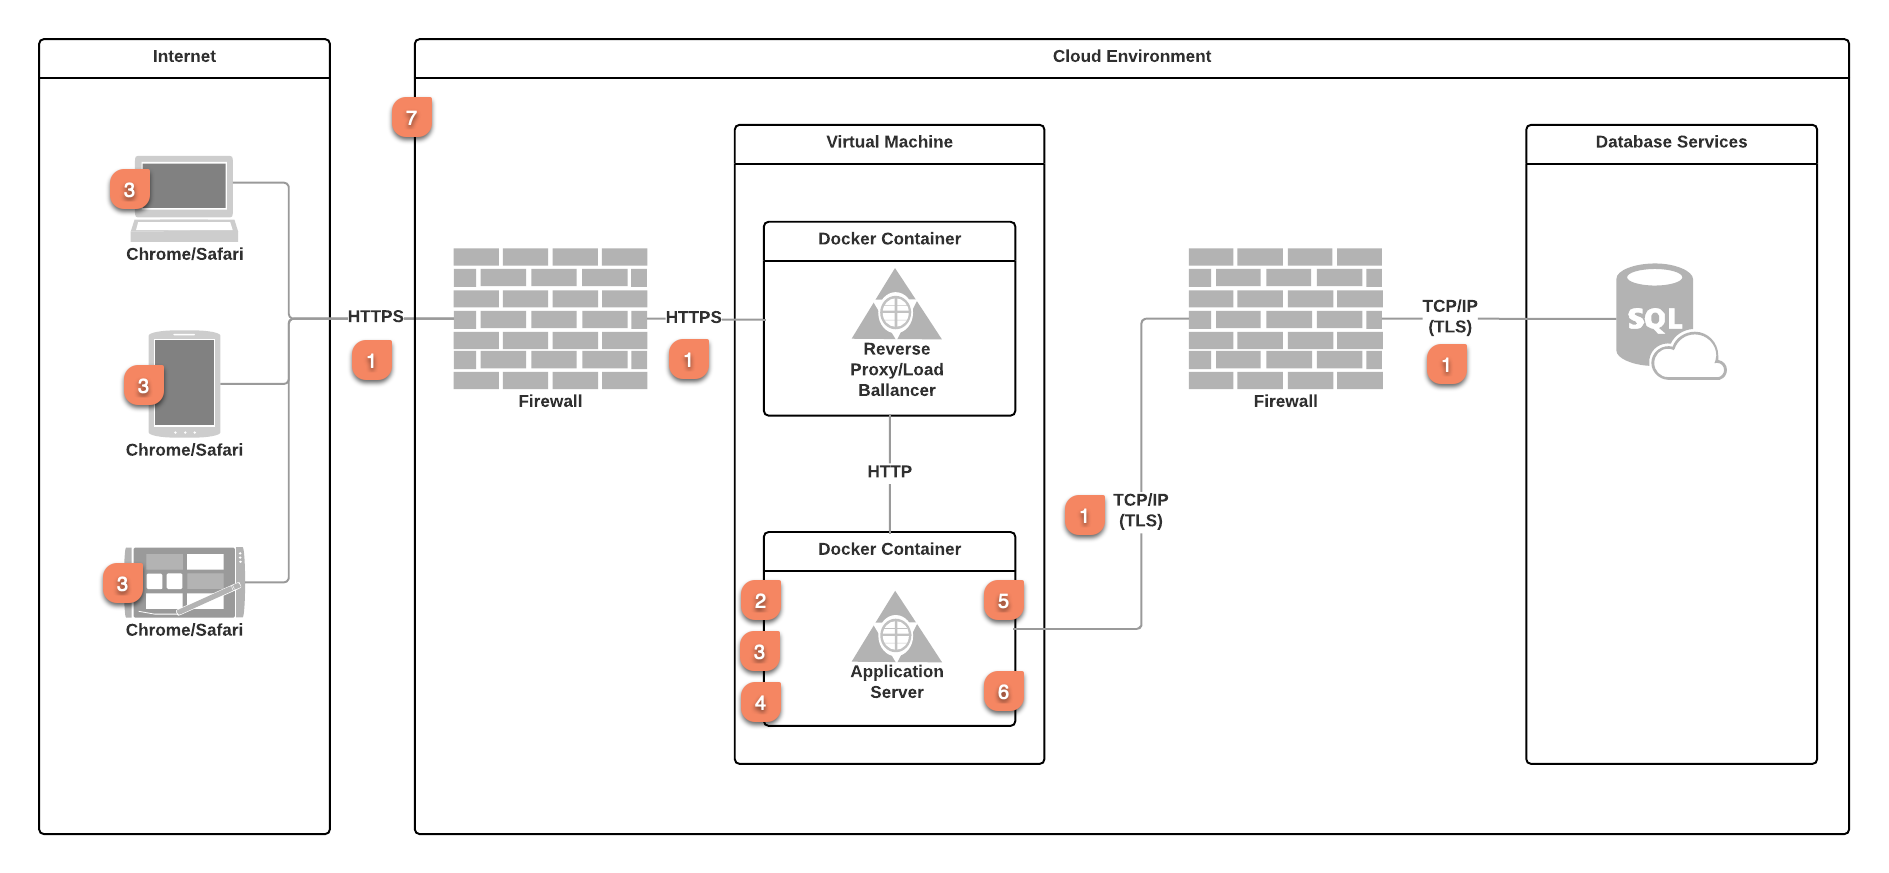
\includegraphics[width=1\linewidth]{images/01-security-diagram.png}
	\caption{A high-level security diagram for TG applications.}\label{sec:01:fig:1}
	\end{figure}

\section*{Secure communication and authentication}\label{sec:02}

\subsection*{Server Authentication for User Protection}

	Application users should be certain that they are accessing the right application on the correct server, and that their communication with the server is secure.
	This basically means three things:

	\begin{itemize}
	\item The server is \emph{authentic}.
	\item The \emph{data integrity} of the communicated information is ensured.
	\item The communication channel is \emph{encrypted}.
	\end{itemize}

	The HTTP protocol over TLS (Transport Layer Security, aka SSL, Secure Sockets Layer) provides a complete solution to the above requirements.
	Thus, the HTTPS protocol support by the TG Application 	Server is the most rigorous solution to the problem of Server Authentication.

\subsubsection*{How HTTPS works}
	Without going too much into the details, it is beneficial to have a general understanding of the HTTPS security and how it actually makes communication safe.
	There are two parts to the TLS mechanism.
	One has to do with encrypting the communication channel, another has to do with certification, which identifies the server as the entity it claims to be. Let's start with channel encryption.

	\paragraph{Channel encryption.}
	The TLS clockwork employs the use of Asymmetric~\cite{PKC} and Symmetric~\cite{SKC} Cryptography.
	The asymmetric cryptography uses two keys -- public and private -- for encryption/decryption of messages.
	If a messages gets encrypted with a private key it can only be decrypted with corresponding public key and wise versa.
	The public key, as the name suggests, gets send to the client application (e.g. a web browser) via an open channel.
	Any eavesdropping adversary would be able to see it, and that is completely fine. The private key remains private to the server.
	So, unless the server is hacked, only the server should be in a possession of the private key.

	Thus, once the client received a public key, all the information encrypted by the client and send back to the server can only be decrypted at by the server.
	However, any information encrypted and send by the server can be decrypted not only by the client, but also by the eavesdropping adversary, who might have captured the public key during its initial transmission to the client.

	This is where the symmetric cryptography comes into place.
	Symmetric cryptography uses a single key for encoding/decoding, and is much faster than asymmetric cryptography at that.
	Therefore, upon receiving a public key, the client generates a key for symmetric cryptography, encodes it with its public key and sends back to the server.
	Thus provided key for symmetric cryptography would only be decrypted at the server end.
	At this stage both client and server have a shared key and start using it to encode/decode all further communication.
	No eavesdropping adversary would not be able to understand any of the information being communicated this way.

	\paragraph{Server Certification.}
	Another part of the TLS clockwork has to do with server identification, and this is where certification plays its role.
	As part of the HTTPS handshake between the client and server, the server presents a certificate of authenticity.
	This certificate has to be signed by a Certificate Authority (CA) or it could be self signed.

	The client such as a web browser has means for checking whether it can trust the presented certificate.
	If the certificate is signed by some CA, the client checks agains its reference of trusted CAs and if make a decision to trust or not to trust the presented certificate.
	If the certificate is self signed, all web browsers reject such certificate unless it was added to a list of exceptions (i.e. the user explicitly informed the browser to trust this certificate).

	If the certificate is rejected then all communication with the server is stopped, as it could be an imposter trying to emulate the actual server that the client intends to connect to.
	However, if the certificate is accepted, the client carries out with a HTTPS handshake (exchanges the keys etc.).

	An interesting thing about CAs is that any organisation (or person for that matter) could become a CA and start signing, for example, its server certificates.
	Customers may choose to trust a particular not well known CA (e.g. FMS) by adding a corresponding CA certificate to their OS or browser.
	So, this all boils down to the trust, and has nothing to do with the actual encryption of the communication channel.

	Please note that each server certificate is issued for a single fully qualified domain name (FQDN).
	This information is used by browser to check that the FQDN part of the URI they are accessing matches the \texttt{Common Name} property of the presented certificate.
	Certificates for different servers should always be issued by signing Public/Private Keys that are unique to those servers (i.e. no server certificate should reuse the same key pair).

\subsubsection*{Communication over HTTPS}

	\paragraph{Java KeyStore.}
	Jetty, which is a Servlet Engine and a HTTP Server used as the basis for TG Application Server, together with Restlet (a framework used for implementing Resource Oriented architecture of TG Application Server) support TLS infrastructure, and can be configured to enable communication over HTTPS.

	A Java KeyStore (JKS) infrastructure is used for that (as in case of any Java application) to establish a TLS infrastructure.
	The server Public/Private Keys and its Certificate, which are used to establish a HTTPS communication, are stored in a keystore file.
	A keystore file should be protected by a password. Access to Private Keys, which are stored there, are also protected by yet another password.

	The keystore file password is mainly used to check file integrity when accessing it in order to make sure that it was not tempered with.
	Also, it provides an additional layer of protection is case the keystore file gets leaked/stolen.
	The Private Key password is there to protect the Private Keys that are stored in a keystore file.
	This introduces yet another security layer to protect the most essential information, which is used for establishing secure communication between the client and server software.
	It a keystore gets stolen and cracked then eavesdropping adversaries in possession of this information would easily read all communication, and could even set up a fake server to obtain user names and passwords by redirecting users to thus set up service.

	In most cases, the keystore file is located on the same physical server as the application server, and is protected by the underlying OS.
	Thus, if the server security is sound there would be no way to steal the keystore file.

	Another important concern is how to handle passwords to a keystore file and Private Keys.
	One common anti-pattern is to store those passwords in a class file as part of the source.
	This leads to two possible ways for an adversary to access the passwords.
	Firstly, the application source might get stolen (e.g. a GitHub repo gets hacked).
	In this case an adversary would obtain the passwords from the source files.
	Secondly, packed jar files of the application server might get leaked as a result of some (even accidental) security breach (e.g. jar files got uploaded to an insecure FTP server).
	By decompiling classes from jars, an adversary would obtain the passwords.

	The most reasonable option is to provide those password as an application server parameter during its start up.
	Securing application configurations falls into the domain of the configuration management, and is usually specific to a deployment environment.

	In addition, different TLS certificates are used for development and deployment purposes, and kept in different keystore files.
	In fact, the deployment keystore file should only be kept at the deployment server, and it would be best if the only person who knows the password to that keystore and Public Keys is the administrator of the deployment server.
	This way any accidental information leaks would be significantly reduced.

	\paragraph{Let's Encrypt.}
	An alternative to maintaining JKS files, it to use Let's Encrypt -- a non-profit certificate authority that provides X.509 certificates for TLS at no charge~\cite{LEC}.
	This approach is arguable more secure and easier to maintain due to an automated process for certificate renewal.
	Also, using this approach fosters better modularity by moving responsibility for maintaining the TLS infrastructure away from the application.
	For example, a reverse proxy such as HA Proxy, can be responsible for maintaining the TLS infrastructure.
	This approached proved to be reliable in real life production deployments of TG applications, and is recommended as a default option.


\subsection*{Client Authentication for Server Protection}

	The previous section describes a way to protect the user from connecting to an untrusted server and from eavesdropping adversary listening to the data being exchanged.
	This, however, does not protect the server from being accessed by an interrogative adversary, who would want to access the data that is stored at the server side.
	There are no bullet proof methods agains user imposters, but there are approaches that would most certainly make it really challenging to break.

	If a server needs to be protected from anonymous access, a client authentication mechanism would need to be put in place.
	Unfortunately, unlike in case of HTTPS, there are no standard reliable HTTP mechanisms for user authentication.
	However, there are very reasonable approaches on top of HTTP that proved to be highly reliable.
	Article ``Dos and Don’ts of Client Authentication on the Web''~\cite{MIT} by MIT Laboratory for Computer Science provides a really good insight into the problem with client authentication and offers one possible solution that was well analysed from different penetration perspectives.
	TG employs the system based on the proposed approach, but with its own modification to further hardens the schema.

	The rest of the discussion is presented in several subsections, each addressing specific concerns of the developed methodology for client authentication.

\subsubsection*{Login and 2-factor authentication}
	It is assumed that before the first time any user attempts to login to the system, they've been registered by a system administrator and have been provided with their username.
	No passwords are specified for such first time users.

	When users access the system, they are presented with a login prompt where they can sing in by entering their credentials or, as it would be in case of first time users, choose to sign up.
	The sign up functionality provides users with a prompt to enter their username (provided to them by a system administrator) and the password of their choosing (see more regarding this in the next subsection).

	In order to validate that the person who is signing up is in fact a valid user and not an imposter, a cryptographically random token gets send to user's email and should be presented by the user to complete the sigh up process.
	As the result of successful sign up, user's system record gets updated with a HMAC-SHA1 hash code of the password.

	Once user is signed up, s/he is required to login explicitly.
	Each explicit login can done in conjunction with 2-factor authentication~(2FA), where the user should enter a one-time passcode generated using HOTP~\cite{HOTP} or TOTP~\cite{TOTP} algorithms.
	The delivery mechanism for passcodes could be an SMS or a mobile app such as Google Authenticator.
	Alternatively, if neither SMS capability nor mobile authentication app is available, there could always be a weaker 1.5-factor authentication put in place, whereby passcodes are provided to users via email.

	Upon login, the user may choose to mark the device that is used for accessing the application as trusted.
	This tells the system not to require explicit login on this device in future.
	More about this capability is discussed in later sections.

\paragraph*{Password strength}
	The resilience of user passwords to guessing is one of the essential security aspects.
	If user passwords can be easily guessed then no matter how clever and bullet proof is the rest of the application security subsystem, an adversary would have one less barrier to break before gaining access to the application.
	This would be almost like having no user passwords at all.
	The 2-factor authentication makes this a bit harder for an adversary to use the password without the access to user's phone, but through social engineering this kind of information can also be obtained.
	Therefore, it is best to all parts of the security puzzle to be really hard to break or guess.

	There are information entropy based approaches to measuring the strength of passwords (e.g.~\cite{NIST}, \cite{DROPBOX}).
	This approach is both stronger and easier to follow by users comparing to rule-based approaches.
	The lower threshold for the password strength in TG applications is configurable.
	
	The strength of user passwords is only checked when users sing up or change their passwords.
	Password strength is checked at both the client and the server sides.
	At the client side users are provided with an instantaneous strength estimation feedback upon entering their password.
	\hyperref[sec:02:fig:1]{Fig.~\ref*{sec:02:fig:1}} illustrates a situation where password, entered by the user, was recognised as ``strong''.
	This way users know that their passwords are reliable and would not be rejected by the server upon submit.

	\begin{figure}[h!tbp]
	\centering
	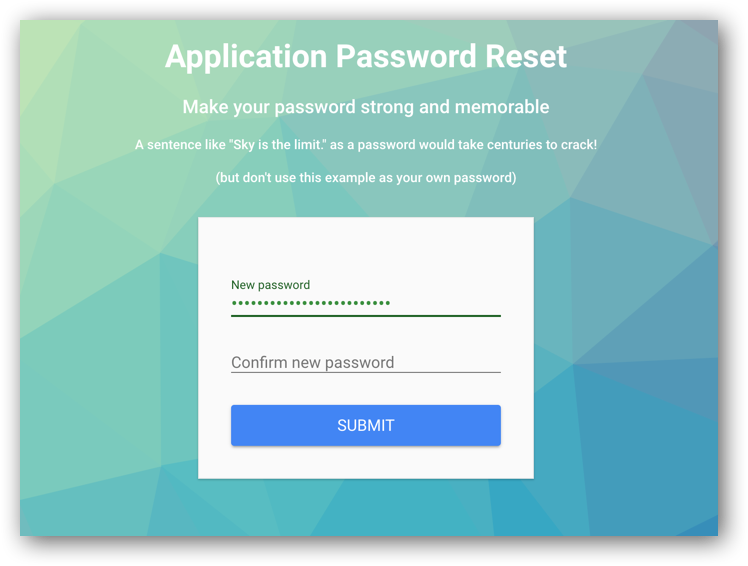
\includegraphics[width=0.7\linewidth]{images/03-new-user-setting-up-password.png}
	\caption{Password strength indication.}\label{sec:02:fig:1}
	\end{figure}

\paragraph*{Preventing rapid-fire login attempts}

\subsubsection*{Restoring a password}


\subsubsection*{Reduced Sign-On instead of Single Sign-On}

\paragraph*{Authenticators}


\subsection*{Securing communication between applications and databases}


\section*{Authorisation}\label{sec:03}

\subsection*{User roles and security tokens}

\paragraph{Security Matrix.}

\section*{User-driven data filtering}

\section*{Deployment environment and its security}\label{sec:04}

%
% ---- Bibliography ----
%
\begin{thebibliography}{5}

\bibitem{PKC} Public Key Cryptography,
\href{http://en.wikipedia.org/wiki/Public-key_cryptography}{Online}

\bibitem{SKC} Symmetric Key Cryptography,
\href{http://en.wikipedia.org/wiki/Symmetric-key_algorithm}{Online}

\bibitem{LEC} Let's Encrypt,
\href{https://letsencrypt.org}{Online}

\bibitem{MIT} Dos and Don'ts of Client Authentication on the Web,
\href{https://pdos.csail.mit.edu/papers/webauth:sec10.pdf}{Online}

\bibitem{HOTP} HMAC-based one-time password algorithm,
\href{https://en.wikipedia.org/wiki/HMAC-based_One-time_Password_algorithm}{Online}

\bibitem{TOTP} Time-based one-time password algorithm,
\href{https://en.wikipedia.org/wiki/Time-based_One-time_Password_algorithm}{Online}

\bibitem{NIST} Password strength: NIST special publication 800-63,
\href{http://en.wikipedia.org/wiki/Password_strength#NIST_Special_Publication_800-63}{Online}

\bibitem{DROPBOX} Dropbox approach to passwords,
\href{https://blogs.dropbox.com/tech/2012/04/zxcvbn-realistic-password-strength-estimation}{Online}


\end{thebibliography}
%

\end{document}

